%%%%%%%%%%%%%%%%%%%%%%%%%%%%%%%% COMMENT THIS TO COMPILE main.tex %%%%%%%%%%%%%%%%%%%%%%%%%%%%%%%%
\documentclass[a4paper,12pt]{report}
\usepackage[english]{babel}
\usepackage[left=2cm,right=2cm,top=2cm,bottom=2cm]{geometry}
%\usepackage{mathtools}
\usepackage{amsthm}     % for definitions and theorems
\usepackage[many]{tcolorbox}    % boxes around definitions and theorems
%\usepackage{amsmath}
%\usepackage{nccmath}
\usepackage{amssymb}    % \ltimes
\usepackage{etoolbox}   % for start of Chapter
%\usepackage{amsfonts}
\usepackage{physics}    % for all Physics related
\usepackage{dsfont}     % for the identity matrix symbol \1
%\usepackage{mathrsfs}

\usepackage{titling}
\usepackage{indentfirst}

\usepackage{bm}
\usepackage[dvipsnames]{xcolor}
\usepackage{cancel}

\usepackage{xurl}
\usepackage[colorlinks=true]{hyperref}

\usepackage{float}
\usepackage{graphicx}
\usepackage{subcaption}
%\usepackage{tikz}

\usepackage{ctable}     % tabelas
\renewcommand{\P}{\phantom{+}}  % empty space to indent things
\usepackage{multirow}
\usepackage{tabulary}

%%%%%%%%%%%%%%%%%%%%%%%%%%%%%%%%%%%%%%%%%%%%%%%%%%%

\newcommand{\eps}{\epsilon}
\newcommand{\vphi}{\varphi}
\newcommand{\cte}{\text{cte}}

\newcommand{\N}{{\mathbb{N}}}
\newcommand{\Z}{{\mathbb{Z}}}
%\newcommand{\Q}{{\mathbb{Q}}}
\newcommand{\C}{{\mathbb{C}}}
\renewcommand{\S}{{\hat{S}}}
%\renewcommand{\H}{\s{H}}

\renewcommand{\a}{{\vb{a}}}
\renewcommand{\b}{{\vb{b}}}
\renewcommand{\d}{{\dagger}}
\newcommand{\up}{{\uparrow}}
\newcommand{\down}{{\downarrow}}
\newcommand{\hc}{{\text{h.c.}}}

\newcommand{\ihat}{\bm{\hat{\imath}}}
\newcommand{\jhat}{\bm{\hat{\jmath}}}
\newcommand{\khat}{\bm{\hat{k}}}

\newcommand{\0}{{\vb{0}}}
\newcommand{\1}{\mathds{1}}
\newcommand{\E}{{\vb{E}}}
\newcommand{\B}{{\vb{B}}}
\renewcommand{\u}{{\vb{u}}}
\renewcommand{\v}{{\vb{v}}}
\renewcommand{\r}{{\vb{r}}}
\newcommand{\R}{{\vb{R}}}
\newcommand{\Q}{{\vb{Q}}}
\newcommand{\G}{{\vb{G}}}
\newcommand{\g}{{\vb{g}}}
\renewcommand{\k}{{\vb{k}}}
\newcommand{\K}{{\vb{K}}}
\newcommand{\p}{{\vb{p}}}
\newcommand{\q}{{\vb{q}}}
\newcommand{\F}{{\vb{F}}}
\renewcommand{\t}{{\vb{t}}}
\newcommand{\vtau}{{\bm{\tau}}}
\newcommand{\vdelta}{{\bm{\delta}}}

% COLORED SYMMETRY ELEMENTS
\newcommand{\Ct}{{\textcolor{Cyan}{C_3}}}
\newcommand{\Ctn}[1]{{\textcolor{Cyan}{C_3^{\textcolor{black}{#1}}}}}
\newcommand{\Cs}{{\textcolor{ForestGreen}{C_6}}}
\newcommand{\Csn}[1]{{\textcolor{ForestGreen}{C_6^{\textcolor{black}{#1}}}}}
\newcommand{\sd}{{\textcolor{RoyalBlue}{\sigma_d}}}
\newcommand{\sdn}[1]{{\textcolor{RoyalBlue}{\sigma_d^{\textcolor{black}{#1}}}}}
\newcommand{\sdp}{{\textcolor{RoyalBlue}{\sigma_d'}}}
\newcommand{\sdpp}{{\textcolor{RoyalBlue}{\sigma_d''}}}
\newcommand{\sv}{{\textcolor{Orange}{\sigma_v}}}
\newcommand{\svn}[1]{{\textcolor{Orange}{\sigma_v^{\textcolor{black}{#1}}}}}
\newcommand{\svp}{{\textcolor{Orange}{\sigma_v'}}}
\newcommand{\svpp}{{\textcolor{Orange}{\sigma_v''}}}

\newcommand{\s}{\sigma}
%\newcommand{\prodint}[2]{\left\langle #1 , #2 \right\rangle}
\newcommand{\cc}[1]{\overline{#1}}
\newcommand{\Eval}[3]{\eval{\left( #1 \right)}_{#2}^{#3}}
\newcommand{\sg}[2]{\{ #1 \mid #2 \}}

\newcommand{\unit}[1]{\; \mathrm{#1}}

\newcommand{\n}{\medskip}
\newcommand{\e}{\quad \mathrm{and} \quad}
\newcommand{\ou}{\quad \mathrm{or} \quad}
\newcommand{\virg}{\, , \;}
\newcommand{\ptodo}{\forall \,}
\renewcommand{\implies}{\; \Rightarrow \;}
%\newcommand{\eqname}[1]{\tag*{#1}} % Tag equation with name

\setlength{\droptitle}{-7em}

\makeatletter
\patchcmd{\chapter}{\if@openright\cleardoublepage\else\clearpage\fi}{}{}{}  % start 'Chapter' at the same page. needs package etoolbox
\makeatother

%% Theorems, definitions, proofs
\theoremstyle{definition}

\newtheorem{definition}{Definition}[section]
\tcolorboxenvironment{definition}{
  colback=blue!5!white,
  boxrule=0pt,
  boxsep=1pt,
  left=2pt,right=2pt,top=2pt,bottom=2pt,
  oversize=2pt,
  sharp corners,
  before skip=\topsep,
  after skip=\topsep,
}

\newtheorem{theorem}{Theorem}[section]
\tcolorboxenvironment{theorem}{
  colback=blue!5!white,
  boxrule=0pt,
  boxsep=1pt,
  left=2pt,right=2pt,top=2pt,bottom=2pt,
  oversize=2pt,
  sharp corners,
  before skip=\topsep,
  after skip=\topsep,
}

\begin{document}
%%%%%%%%%%%%%%%%%%%%%%%%%%%%%%%% COMMENT THIS TO COMPILE main.tex %%%%%%%%%%%%%%%%%%%%%%%%%%%%%%%%


%%%%%%%%%%%%%%%%%%%%%%%%%%%%%%%%%%%%%%%%%%%%%%%%%%%%%%%%%%%%%%%%%%%%%%%%%%%%%%%%%%%%%%%%%%%%%%%%%%
\chapter{Emmergent symmetries and Wannier obstruction in TBG} \label{ch:emmergent_symm_wannier_obstruction}
%%%%%%%%%%%%%%%%%%%%%%%%%%%%%%%%%%%%%%%%%%%%%%%%%%%%%%%%%%%%%%%%%%%%%%%%%%%%%%%%%%%%%%%%%%%%%%%%%%

%%%%%%%%%%%%%%%%%%%%%%%%%%%%%%%%%%%%%%%%%%%%%%%%%%%%%%%%%%%%%%%%%%%%%%%%%%%%%%%%%%%%%%%%%%%%%%%%%%
\section{Commensurate structures} \label{sec:tbg_commensurate}
%%%%%%%%%%%%%%%%%%%%%%%%%%%%%%%%%%%%%%%%%%%%%%%%%%%%%%%%%%%%%%%%%%%%%%%%%%%%%%%%%%%%%%%%%%%%%%%%%%

Twisted bilayer graphene (TBG) features two graphene layers rotated relative to each other by an angle \( \theta \). This rotation gives rise to a moiré pattern, formed by the interference of the two lattices. The pattern can be either \textit{commensurate}, exhibiting translational symmetry and forming a periodic superlattice, or \textit{incommensurate}, lacking translational symmetry and periodicity. Figure \ref{fig:moireD6} illustrates a commensurate moiré pattern with \( D_6 \) point group symmetry, where the rotation center lies at the center of a hexagon. The AA, AB, and BA regions in the pattern represent areas where \( A \) or \( B \) carbon atoms from the layers align with each other.

The system can generally exhibit different symmetry groups depending on the choice of the origin for the rotation by \( \theta \). However, the largest possible point group is \( D_6 \), due to the honeycomb Bravais lattice of the two layers. In the commensurate case, the primitive lattice vectors \( \vb{L}_1 \) and \( \vb{L}_2 \) are defined as the least common multiples of the unit vectors of the monolayers. Figure \ref{fig:latvec} provides an example for \( \theta = 21.8^\circ \).
\begin{figure}[H]
\centering
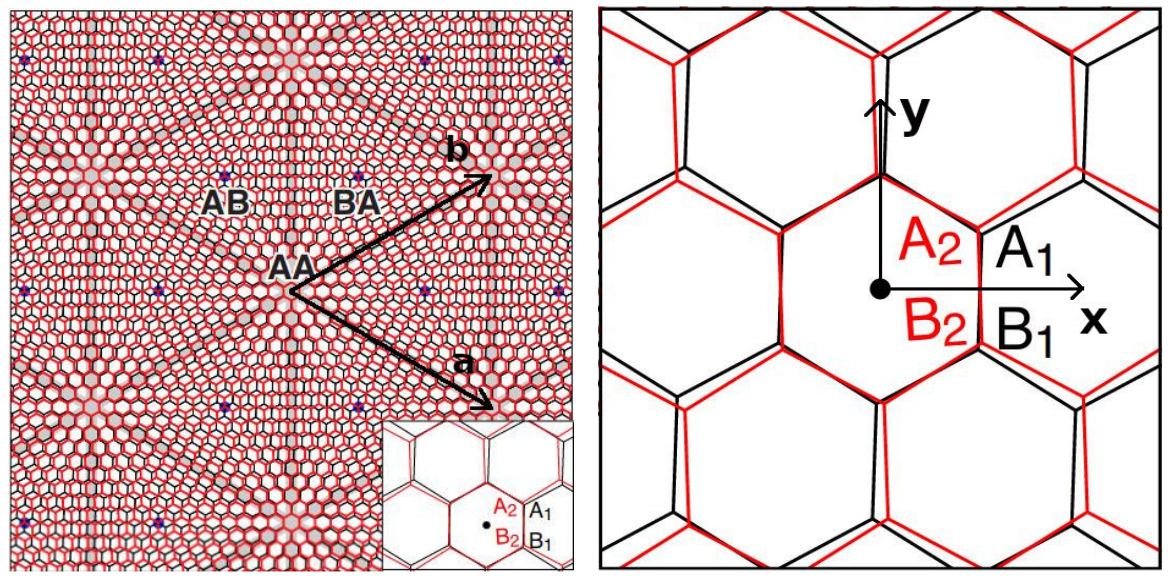
\includegraphics[height=.32\columnwidth]{fig/moireD6.png}
\caption{Commensurate $D_6$-type structure obtained by twisting the two layers from the initial AA stacking configuration, with the origin chosen as the center of the hexagons. Figure taken from \cite{thesis_rennella}.}
\label{fig:moireD6}
\end{figure}

%As drawn in Figure \ref{fig:latvec}, we have
%\begin{align}
%\label{eq:scalarprods1}
%\vb{a}_1^{(1)} \vdot \vb{a}_2^{(1)} &= a^2 \cos(60^\circ) = a^2/2; \\
%\label{eq:scalarprods2}
%\vb{a}_1^{(1)} \vdot \vb{a}_1^{(2)} &= a^2 \cos\theta; \\
%\label{eq:scalarprods3}
%\vb{a}_1^{(1)} \vdot \vb{a}_2^{(2)} &= a^2 \cos(60^\circ + \theta); \\
%\label{eq:scalarprods4}
%\vb{a}_1^{(2)} \vdot \vb{a}_2^{(1)} &= a^2 \cos(60^\circ - \theta).
%\end{align}

The superlattice vectors $\vb{L}_1$, $\vb{L}_2$ are related by a $60^\circ$ rotation. In general, because $\vb{L}_1$ belongs to the lattices of both layers, it can be parameterized by integers $n_1^{(1)}, n_2^{(1)}, n_1^{(2)}, n_2^{(2)}$ as
\begin{equation} \label{eq:L1}
\vb{L}_1 = n_1^{(1)}\vb{a}_1^{(1)} + n_2^{(1)}\vb{a}_2^{(1)} = n_1^{(2)}\vb{a}_1^{(2)} + n_2^{(2)}\vb{a}_2^{(2)},
\end{equation}
where $\vb{a}_{1,2}^{(\ell)}$ are the unit vectors of layer $\ell = 1,2$.

The resulting crystal will exhibit exact lattice translational symmetry with the superlattice vectors \( \vb{L}_1 \) and \( \vb{L}_2 \) only if \( \theta \) satisfies the commensurability condition \cite{thesis_rennella, zou2018}, given by integers \( m \) and \( r \):

\begin{equation} \label{eq:costheta}
\cos\theta(m,r) = \frac{3m^2 + 3mr + r^2/2}{3m^2 + 3mr + r^2} = \frac{3 + 3 \qty(\frac{r}{m}) + \frac{1}{2} \qty(\frac{r}{m})^2}{3 + 3 \qty(\frac{r}{m}) + \qty(\frac{r}{m})^2}.
\end{equation}

We point out that \( \theta(m,r) \) is a function of only the ratio \( r/m \) and is monotonic within the range \( 0 \leq \theta \leq 60^\circ \). Therefore, all commensurate angles can be uniquely determined by pairs of coprime integers \( (m, r) \), where \( \gcd(m, r) = 1 \).

There are two types of structures, classified as Type I and Type II \cite{zou2018} (or SE-odd and SE-even, respectively, with SE standing for sublattice exchange \cite{continuum_model_lopesdossantos2012}), each characterized by distinct relationships between the superlattice vectors \(\vb{L}_1\) and \(\vb{L}_2\) and the primitive vectors of the layers. These relationships can be expressed in terms of the primitive vectors of the first layer, \(\a_1^{(1)}\) and \(\a_2^{(1)}\), as follows:
\begin{itemize}

\item \textit{Type I (SE-odd)}, when $\gcd(r, 3) = 1$:
\begin{equation} \label{eq:type-I-L1L2}
\begin{pmatrix}
\vb{L}_1 \\ \vb{L}_2
\end{pmatrix} =
%\begin{pmatrix}
%1 & -1 \\
%1 & 0
%\end{pmatrix}
%\begin{pmatrix}
%m & 2m+r \\
%-(m+r) & m
%\end{pmatrix}
%\begin{pmatrix}
%1 & 0 \\
%-1 & 1
%\end{pmatrix}
%\begin{pmatrix}
%\a_1^* \\ \a_2^*
%\end{pmatrix}
%=
\begin{pmatrix}
m & m+r \\
-(m+r) & 2m+r
\end{pmatrix}
\begin{pmatrix}
\a_1^{(1)} \\ \a_2^{(2)}
\end{pmatrix}.
\end{equation}

\item \textit{Type II (SE-even)} when $\gcd(r,3) = 3$:

\begin{equation} \label{eq:type-II-L1L2}
\begin{pmatrix}
\vb{L}_1 \\ \vb{L}_2
\end{pmatrix} =
%\begin{pmatrix}
%1 & -1 \\
%1 & 0
%\end{pmatrix}
%\begin{pmatrix}
%m+\frac{r}{3} & m+\frac{2r}{3} \\
%-\frac{r}{3} & m+\frac{r}{3}
%\end{pmatrix}
%\begin{pmatrix}
%1 & 0 \\
%-1 & 1
%\end{pmatrix}
%\begin{pmatrix}
%\a_1^{*} \\ \a_2^{*}
%\end{pmatrix}
%=
\begin{pmatrix}
m+\frac{r}{3} & \frac{r}{3} \\
-\frac{r}{3} & m+\frac{2r}{3}
\end{pmatrix}
\begin{pmatrix}
\a_1^{(1)} \\ \a_2^{(2)}
\end{pmatrix}.
\end{equation}

\end{itemize}

For both Type I and Type II structures, the moiré lattice constant \( L(m, r) = \abs{\vb{L}_1} = \abs{\vb{L}_2} \) is determined by the following formula:
\begin{equation} \label{eq:commensurate-constant}
L(m, r) = a \sqrt{\frac{3m^2 + 3mr + r^2}{\gcd(r, 3)}} = \frac{r}{\sqrt{\gcd(r,3)}} \cdot \frac{a}{2 \sin(\theta(m,r)/2)},
\end{equation}
where \(a = 0.246 \unit{nm}\) is the lattice constant of the monolayer, and \(\gcd(r, 3)\) accounts for the sublattice exchange parity.

The unit cell of the moiré superlattice has an area given by
\begin{equation} \label{eq:superlattice_area_unitcell}
A_{\text{moiré}} = \frac{\sqrt{3}}{2} L^2,
\end{equation}
where \( A_1 = \frac{\sqrt{3}}{2} \, a^2 \) represents the area of the unit cell of monolayer graphene. As the angle \( \theta \) decreases, \( A_{\text{moiré}} \) increases significantly. For the magic angle \( \theta \approx 1.1^\circ \), the number of atoms in the moiré unit cell reaches approximately 11,000. As the moiré unit cell expands, its corresponding Brillouin Zone shrinks, forming the mini Brillouin Zone (mBZ). The area of the mBZ is given by
\begin{equation} \label{eq:bz-volume}
\Omega_{\text{mBZ}} = \frac{(2\pi)^2}{A_{\text{moiré}}} = \frac{\gcd(r,3)}{3m^2 + 3mr + r^2} \, \Omega_1,
\end{equation}
where \( \Omega_1 = \frac{(2\pi)^2}{A_1} \) is the area of the monolayer's BZ.

For instance, when \( (m, r) = (1, 1) \), we have \( \gcd(r,3) = 1 \) (Type I structure) and a corresponding twist angle \( \theta(1,1) = 21.8^\circ \). In this case, \( 3m^2 + 3mr + r^2 = 7 \), meaning that the monolayer BZ accommodates 7 mBZs within its area, as illustrated in Figure \ref{fig:bzminibz}.

\begin{figure}[H]
\centering
\begin{subfigure}{.5\textwidth}
  \centering
  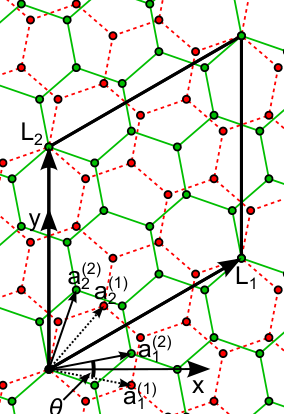
\includegraphics[height=.6\linewidth]{fig/latvec.png}
  \caption{}
  \label{fig:latvec}
\end{subfigure}%
\begin{subfigure}{.5\textwidth}
  \centering
  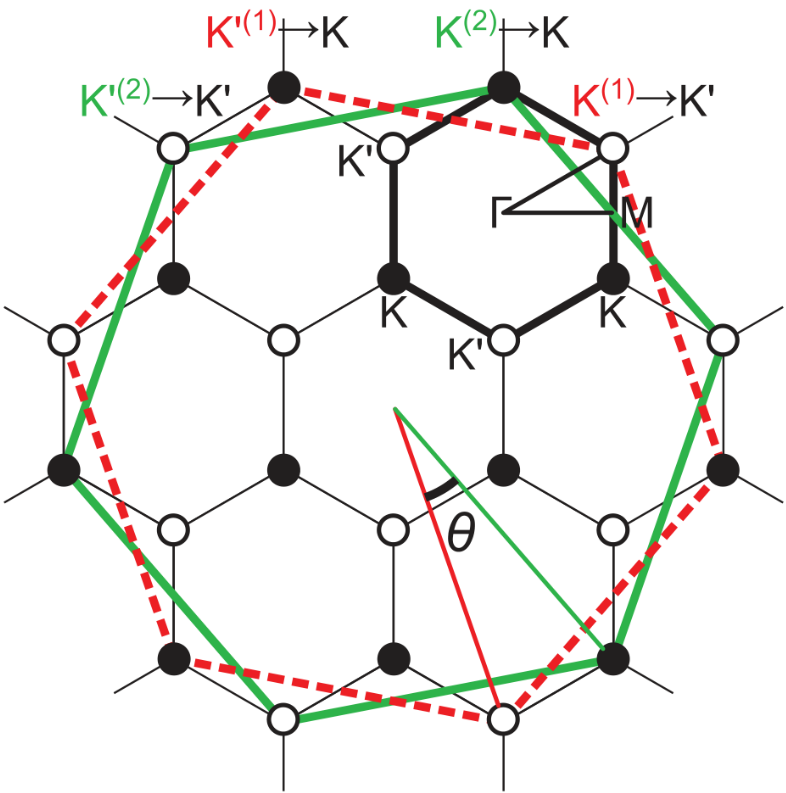
\includegraphics[height=.6\linewidth]{fig/bzminibz.png}
  \caption{}
  \label{fig:bzminibz}
\end{subfigure}
\caption{(a) Commensurate structure and lattice vectors $\vb{L}_1$, $\vb{L}_2$. (b) Monolayers (red and green) and mini BZ's with $(m,r) = (1,1)$ and $\theta = 21.8^\circ$. Figures taken from \cite{koshino2012}. %\textbf{SEPARAR AS FIGURAS}
}
\label{fig:geometry}
\end{figure}

The distinct relationships between the superlattice vectors for Type I and Type II structures lead to different folding patterns for the Dirac points \(K_1\) and \(K_2\) of the monolayers into the mBZ. For example, in Type I structures, the Dirac points \(K_1\) and \(K_2\) fold into different valleys in the mBZ, with \(K_1\) folding to \(K_m'\) and \(K_2\) folding to \(K_m\), as illustrated in Figure \ref{fig:bzminibz}. In contrast, for Type II structures, \(K_1\) and \(K_2\) fold into the same type of Dirac point, \(K_m\), in the mBZ. For a more detailed discussion of these folding patterns, refer to \cite{zou2018}.


We emphasize that the commensuration condition for TBG depends only on the twist angle $\theta$, not the twisting center. As long as the twist angle satisfies Equation \ref{eq:costheta}, the bilayer retains exact translational symmetry, even if the twisting center is a generic point where no two carbon atoms align perfectly. The moiré lattice vectors $\vb{L}_1$ and $\vb{L}_2$, lattice constant \( L(m, r) \), and momentum mapping between the microscopic and moiré Brillouin zones depend solely on the twist angle and not the twisting center. However, the twisting center determines the exact point-group symmetries of the commensurate lattice. If the twisting center is a generic point, translations are the only exact spatial symmetries. If it is the center of a hexagon as in Figure \ref{fig:moireD6}, the twisted bilayer graphene inherits the six-fold rotational symmetry \( C_6 \) of the monolayers.

%%%%%%%%%%%%%%%%%%%%%%%%%%%%%%%%%%%%%%%%%%%%%%%%%%%%%%%%%%%%%%%%%%%%%%%%%%%%%%%%%%%%%%%%%%%%%%%%%%
\section{Emergent symmetries} \label{sec:emergent_symm}
%%%%%%%%%%%%%%%%%%%%%%%%%%%%%%%%%%%%%%%%%%%%%%%%%%%%%%%%%%%%%%%%%%%%%%%%%%%%%%%%%%%%%%%%%%%%%%%%%%

From the discussion in Section \ref{sec:tbg_commensurate}, one might conclude that a commensurate TBG system should exhibit a translational symmetry with a lattice constant \( L(\theta) \), as given by Eq. \eqref{eq:commensurate-constant}. However, as discussed in \cite{zou2018}, scanning tunneling microscopy (STM) experiments actually observe an effective moiré lattice constant \( L'(\theta) \), which does not depend on whether the system is commensurate or incommensurate. This effective lattice constant is given by
\begin{equation} \label{eq:STM-constant}
L'(\theta) = \frac{a}{2 \sin(\theta/2)} \leq L(\theta).
\end{equation}

This can be interpreted as TBG exhibiting an approximate translational symmetry with superlattice constant $L'(\theta)$, despite optionally possessing an exact translational symmetry with $L(\theta)$ in the commensurate case.

The presence of over 11,000 atoms in the unit cell of MATBG at \( \theta \approx 1.1^\circ \) makes any calculation beyond a simple tight-binding model highly computationally demanding, if not practically infeasible. This issue can be addressed by employing the less computationally intensive Bistritzer-MacDonald (BM) model \cite{macdonald2011}. The Bistritzer-MacDonald model (also known as the ``continuum theory'') incorporates translational symmetry by a lattice constant $L'(\theta)$ and other emergent symmetries observed in TBG experiments. This theory describes the system at every twist angle $\theta \lesssim 10^\circ$, including incommensurate ones \cite{continuum_model_castroneto2007, macdonald2011}. It predicts universal features, such as Dirac crossings between valence and conduction bands in each valley, which match tight-binding calculations for commensurate structures and experimental data for larger twist angles, where correlation effects are less significant \cite{zou2018}.

However, the original Bistritzer-MacDonald model underestimates the gap between the nearly flat bands and the other bands. In a real system, the lattice structure spontaneously relaxes to achieve an energetically favorable configuration. In twisted bilayer graphene (TBG) with a small twist angle, distinct regions of AB/BA and AA stacking emerge. Since the interlayer binding energy is minimized in the AB and BA configurations and maximized in the AA configuration, TBG undergoes in-plane deformation to enhance the AB/BA regions and reduce the AA regions. This structural relaxation alters the electronic band structure, leading to the opening of gaps. The effects of lattice relaxation can be phenomenologically incorporated into the BM model by adjusting its parameters, as demonstrated in previous work \cite{koshinohubbard2018}.

The continuum theory incorporates additional symmetries, such as translations by $L'(\theta)$, rotation \(C_6 T\) and valley \(U_v(1)\) symmetries, which, while not fully realized in commensurate structures, play a crucial role in protecting Dirac points in valley-filtered bands \cite{zou2018}. The \(C_2 T = (C_6 T)^3\) symmetry, in particular, prevents the Dirac points from opening a gap. While these symmetries are approximations, they remain effective down to the energy scales currently accessible in small-angle TBG experiments. As a result, the differences between commensurate and incommensurate structures become negligible in practice.

A key feature of the band structure resulting from the Bistritzer-MacDonald model is the inability to construct well-localized Wannier functions that respect all the model's symmetries. This issue arises because certain symmetries, such as \(C_2 T\) and \(U_v(1)\), are not exact at the microscopic level, but are crucial for preserving Dirac crossings and they alter the topology of the bands. As discussed in Chapter \ref{ch:topological_quantum_chemistry}, this phenomenon is known as a Wannier obstruction, which occurs because the topology of the bands is non-trivial.

In conclusion, the continuum theory offers significant advantages for the description of TBG, such as incorporating the ``good'' emergent symmetries, such translations, \(C_6 T\) and \(U_v(1)\). However, fully implementing these symmetries results in a Wannier obstruction. In Section \ref{sec:BM-model}, we provide a detailed derivation of the BM model, while in Section \ref{sec:wannier_obstruction}, we discuss its associated Wannier obstruction.

%%%%%%%%%%%%%%%%%%%%%%%%%%%%%%%%%%%%%%%%%%%%%%%%%%%%%%%%%%%%%%%%%%%%%%%%%%%%%%%%%%%%%%%%%%%%%%%%%%
\section{Bistritzer-MacDonald model} \label{sec:BM-model}
%%%%%%%%%%%%%%%%%%%%%%%%%%%%%%%%%%%%%%%%%%%%%%%%%%%%%%%%%%%%%%%%%%%%%%%%%%%%%%%%%%%%%%%%%%%%%%%%%%


The atomic 2D positions for each layer $\ell$ of TBG are given by
\begin{equation} \label{eq:position-atoms-tbg}
\r = n_1 \a_{1}^{(\ell)} + n_2 \a_{2}^{(\ell)} + \vtau_{\alpha}^{(\ell)},
\end{equation}
where $\alpha = A, B$ indexes the site type, and $\vtau_{\alpha}^{(\ell)}$ are the basis vectors. The lattice vectors $\a_{j}^{(\ell)}$ are obtained by rotating the unrotated vectors $\a_j$ by an angle $\theta_\ell$ using the rotation matrix $R_{\theta_\ell}$. We use the convention $\a_1 = a(1,0)$ and $\a_2 = a\qty(\frac{1}{2}, \frac{\sqrt{3}}{2})$. The rotation matrix is defined as
\begin{equation} \label{eq:rotation-matrix}
R_\theta =
\begin{pmatrix}
\cos\theta & -\sin\theta \\
\sin\theta & \cos\theta
\end{pmatrix}.
\end{equation}
We choose the reference frame such that $\theta_1 = -\theta/2$ and $\theta_2 = +\theta/2$, with the AA-stacking configuration as the starting position ($\theta=0$). In this configuration, our the twisting center is placed at the center of a hexagon. Before the rotation, the sublattice vectors are $\vtau_A = \frac{\a_1 + \a_2}{3} = d\qty(\frac{\sqrt{3}}{2}, \frac{1}{2})$ and $\vtau_B = \frac{-\a_1 + 2\a_2}{3} = d(0,1)$. The sublattice vectors of each layer after the rotation are then given by
\begin{equation} \label{eq:tau_tbg_lattice_AB}
\vtau_{\alpha}^{(\ell)} = R_{\theta_\ell} \vtau_\alpha.
\end{equation}

The momentum lattice vectors for each layer are expressed as \( \mathbf{b}_j^{(\ell)} = R_{\theta_\ell} \mathbf{b}_j \), where \( \mathbf{b}_{1,2} \) are the reciprocal lattice vectors of the monolayer graphene, as defined in Equation \ref{eq:monolayer-bvecs}. The moiré pattern can be understood as arising from a beat effect \cite{handbook2019}, with the outer beat periodicity determined by the moiré reciprocal lattice vectors
\begin{equation} \label{eq:beat_effect-moire_momentum}
\b_j^{\text{moiré}} = \b_{j}^{(1)} - \b_{j}^{(2)}.
\end{equation}

Under this assumption, \( K_1 \) folds into \( K_m' \) and \( K_2 \) folds into \( K_m \) in the moiré Brillouin zone (mBZ), implying that the Bistritzer-MacDonald (BM) model assumes a Type I (SE-odd) structure if the system were commensurate \cite{thesis_angeli, zou2018}. From Equation \ref{eq:beat_effect-moire_momentum}, the explicit expressions for the moiré momentum lattice vectors are given by:
\begin{equation} \label{eq:moire-bvecs}
\vb{b}_1^{\text{moiré}} = \sqrt{3} k_\theta \qty(-\frac{1}{2}, -\frac{\sqrt{3}}{2}), \quad
\vb{b}_2^{\text{moiré}} = \sqrt{3} k_\theta \qty(1, 0),
\end{equation}
where $k_\theta = \abs{K_1-K_2} = 2 \abs{K} \sin(\theta/2) = \frac{8\pi}{3a} \sin(\theta/2)$.

The BM Hamiltonian $H$ is constructed from a tight-binding approach, $H = H_1 + H_2 + H_{\perp}$, where $H_\ell$ corresponds to the Hamiltonian of layer $\ell$ and $H_\perp = V + V^\d$ accounts for interlayer hybridization. In the Bloch wave basis, the wavefunctions are written as
\begin{equation} \label{eq:BM-blochwave}
\ket{\psi_{\ell, \k, \alpha}} = \frac{1}{\sqrt{N_\ell}} \sum_{\R_\ell} e^{i \k \vdot \qty(\R_\ell + \vtau_{\alpha}^{(\ell)})} \ket{\ell, \R_\ell, \alpha},
\end{equation}
where $\ell$ labels the layer, $N_\ell$ is the number of unit cells, $\R_\ell = n_1 \a_1^{(\ell)} + n_2 \a_2^{(\ell)}$ are the Bravais triangular lattice positions, $\vtau_{\alpha}^{(\ell)}$ are sublattice centers, and $\ket{\ell,\R_\ell,\alpha}$ represents Wannier states.

The Hamiltonian of an unrotated single layer of graphene, in its low-energy Dirac description for a momentum \(\k\) around the \(K\) or \(K' = -K\) point, is given by
\begin{equation} \label{eq:single_layer_dirac_hamil_mono}
H_{\text{mono}}^\zeta(\k) \approx v_F (\k - \zeta K) \vdot \qty(\zeta \s_x, \s_y),
\end{equation}
where $\zeta = \pm 1$ is the valley index ($\zeta = +1$ for $K$ and $\zeta = -1$ for $K = -K$).

The Dirac nodes of each layer $\ell$ are $K_{\ell} = R_{\theta_\ell} K$, and the layers hamiltonians expanded around the Dirac points are:
\begin{equation} \label{eq:single_layer_dirac_hamil_valley}
H_\ell^{\zeta}\qty(\zeta K_\ell + \q) = H_{\text{mono}}^\zeta\qty(R_{\theta_\ell}^{-1}\qty(\zeta K_\ell + \q)) \approx v_F \qty(R_{\theta_\ell}^{-1} \q) \vdot \qty(\zeta \s_x, \s_y) \approx \zeta v_F \q \vdot \qty(\s_x, \zeta \s_y).
\end{equation}

In Equation \ref{eq:single_layer_dirac_hamil_valley}, we make a second approximation by neglecting the \(\theta\)-dependence and effectively assuming \(R_\theta \approx \1\). This approximation, extensively analyzed in \cite{all_magic_angles, bernevig_II_2021}, proves to be accurate and simplifies the mathematical treatment of the system. Notably, it introduces an effective particle-hole symmetry, which plays a crucial for the topology of the bands. The implications of this symmetry will be discussed in Section \ref{sec:wannier_obstruction}.


The hybridization $V$ of the interlayer Hamiltonian in the second quantization formalism is \cite{handbook2019}
\begin{equation} \label{eq:interlayer-hopping}
V = \sum_{\R_1,\alpha,\R_2,\beta} c_{1,\alpha}^\d(\R_1) t_\perp^{\alpha\beta}(\R_1,\R_2) c_{2,\beta}(\R_2), \quad
t_\perp^{\alpha\beta}(\R_1,\R_2) =
\mel{1,\R_1,\alpha}{V}{2,\R_2,\beta}.
\end{equation}

By performing a transformation to momentum space,
\begin{equation} \label{eq:blg-fourier}
c_{\ell,\alpha}^\d(\R_\ell) = \frac{1}{\sqrt{N_\ell}} \sum_{\k_\ell}
e^{-i\k_\ell \vdot \qty(\R_\ell + \vtau_{\alpha}^{(\ell)})} c_{\ell,\alpha}^\d(\k_\ell),
\end{equation}
where the momenta $\k_\ell$ span the Brillouin zone of layer $\ell$, the interlayer hybridization becomes
\begin{equation} \label{eq:interlayer-hopping-kspace}
V = \sum_{\k_1,\alpha,\k_2,\beta} c_{1,\alpha}^\d(\k_1) T^{\alpha\beta}(\k_1,\k_2) c_{2,\beta}(\k_2),
\end{equation}
with
\begin{equation} \label{eq:interlayer-hopping-Tkspace}
T^{\alpha\beta}(\k_1,\k_2) =
\frac{1}{\sqrt{N_1 N_2}} \sum_{\R_1,\R_2} e^{-i\k_1\vdot\qty(\R_1+\vtau_{\alpha}^{(1)})}
t_\perp^{\alpha\beta}(\R_1,\R_2) e^{i\k_2\vdot\qty(\R_2+\vtau_{\beta}^{(2)})}.
\end{equation}

Assuming that the interlayer hopping term \( t_\perp^{\alpha\beta}(\R_1,\R_2) \) depends only on the relative separation of the two orbital centers \cite{macdonald2011}, we can apply a Fourier transformation:
\begin{equation} \label{eq:interlayer-hopping-fourier}
t_\perp^{\alpha\beta}(\R_1,\R_2) = t_\perp^{\alpha\beta}\qty(\R_1+\vtau_{\alpha}^{(1)}-\R_2-\vtau_{\beta}^{(2)}) =
\int \frac{\dd[2]{\p}}{(2\pi)^2} e^{i \p \vdot \qty(\R_1+\vtau_{\alpha}^{(1)}-\R_2-\vtau_{\beta}^{(2)})} t_\perp^{\alpha\beta}(\p).
\end{equation}

Substituting Eq.~\eqref{eq:interlayer-hopping-fourier} into Eq.~\eqref{eq:interlayer-hopping-Tkspace}, we obtain:
\begin{equation} \label{eq:interlayer-hopping-step1}
T^{\alpha\beta}(\k_1,\k_2) =
\frac{1}{\sqrt{N_1 N_2}} \int \frac{\dd[2]{\p}}{(2\pi)^2} \sum_{\R_1} e^{-i(\k_1-\p)\vdot\qty(\R_1+\vtau_{\alpha}^{(1)})}
t_\perp^{\alpha\beta}(\p) \sum_{\R_2} e^{i(\k_2-\p)\vdot\qty(\R_2+\vtau_{\beta}^{(2)})}.
\end{equation}

Using the lattice relation
\begin{equation} \label{eq:delta_lattice_relation}
\sum_{\R_\ell} e^{i \k \vdot \R_\ell} = N_\ell \sum_{\G_\ell} \delta_{\k,\G_\ell},
\end{equation}
where the summation is over the momentum lattice vectors of each layer, \(\G_\ell = m_1 \b_1^{(\ell)} + m_2 \b_2^{(\ell)}\), Equation \eqref{eq:interlayer-hopping-step1} can be rewritten as:
\begin{equation} \label{eq:interlayer-hopping-step2}
T^{\alpha\beta}(\k_1,\k_2) =
\sqrt{N_1 N_2} \int \frac{\dd[2]{\p}}{(2\pi)^2} \sum_{\G_1, \G_2}
e^{-i \G_1 \vdot \vtau_\alpha^{(1)}} t_\perp^{\alpha\beta}(\p) e^{i \G_2\vdot\vtau_\beta^{(2)}}
\delta_{\k_1-\p, \G_1} \delta_{\k_2-\p, \G_2}.
\end{equation}

Using the Dirac delta property
\begin{equation} \label{eq:dirac_delta_2d_property}
\int \dd[2]{\k} \delta_{\k-\k'} = \frac{(2\pi)^2}{A},
\end{equation}
where \(A\) is the total area of the system, we can write:
\begin{equation} \label{eq:interlayer-hopping-step3}
T^{\alpha\beta}(\k_1,\k_2) =
\sqrt{\frac{N_1 N_2}{A^2}} \sum_{\G_1, \G_2}
e^{i \G_1 \vdot \vtau_\alpha^{(1)}} t_\perp^{\alpha\beta}(\k_1+\G_1) e^{-i \G_2\vdot\vtau_\beta^{(2)}}
\delta_{\k_1+\G_1, \k_2+\G_2}.
\end{equation}

Notice that the total area is \(A = N_\ell A_1\), where \(A_1 = \frac{\sqrt{3}}{2} a^2\) represents the unit cell area of both layers. Equation \ref{eq:interlayer-hopping-step3} then simplifies to:
\begin{equation} \label{eq:interlayer-hopping-simplified}
T^{\alpha\beta}(\k_1,\k_2) = \frac{1}{A_1} \sum_{\G_1, \G_2}
e^{i \G_1 \vdot \vtau_\alpha^{(1)}} t_\perp^{\alpha\beta}(\k_1+\G_1) e^{-i \G_2\vdot\vtau_\beta^{(2)}}
\delta_{\k_1+\G_1, \k_2+\G_2}.
\end{equation}

The term $\delta_{\k_1+\G_1, \k_2+\G_2}$ in Eq. \eqref{eq:interlayer-hopping-simplified}, leads to a ``momentum conservation'',
\begin{equation} \label{eq:umklapp_condition}
\k_1 + \G_1 = \k_2 + \G_2,
\end{equation}
which is known as generalized umklapp condition \cite{handbook2019}.


Since both \( A \) and \( B \) sublattice sites in graphene correspond to \( p_z \) orbitals of carbon atoms, it is reasonable to assume that the interlayer hopping term, \( t_\perp^{\alpha\beta}(\mathbf{r}) \), is independent of the sublattice indices \( \alpha \) and \( \beta \). Thus, we write \( t_\perp^{\alpha\beta}(\mathbf{r}) = t_\perp(\mathbf{r}) \). In \cite{macdonald2011}, the behavior of \( t_\perp(\mathbf{r}) \) is characterized using Slater-Koster parameters \cite{tperp-laissardiere2012}, and the Fourier transform \( t_\perp(\mathbf{p}) \) is numerically evaluated via Eq.~\eqref{eq:interlayer-hopping-fourier}. These estimates confirm that \( t_\perp(\mathbf{p}) \) depends only on \( \abs{\mathbf{p}} \) and exhibits exponential decay. This fact is particularly important, as it ensures that only a limited number of umklapp processes contribute significantly to the coupling in Eq.~\eqref{eq:interlayer-hopping-simplified}.

To analyze the low-energy physics of the system, we focus on momentum states \(\k_1\) and \(\k_2\) that lie near their respective Dirac points: \(K_1\) and \(K_1'\) for layer 1, and \(K_2\) and \(K_2'\) for layer 2. The interlayer coupling matrix \(T^{\alpha\beta}(\k_1, \k_2)\) can, in principle, couple states within the same valley across layers or states between opposite valleys. However, the interlayer hopping term \(t_\perp(\mathbf{p})\), as expressed in Eq.~\eqref{eq:interlayer-hopping-simplified}, decays exponentially with \(\abs{\mathbf{p}}\). As a result, the dominant contributions come from terms where \(\abs{\k_1 + \G_1}\) is minimized while satisfying the momentum conservation of Eq.~\eqref{eq:umklapp_condition}.

For small twist angles \(\theta\), the contributions are dominated by intra-valley couplings, as inter-valley couplings become negligibly small. This holds true even though opposite valleys from different layers fold into the same point in the moiré Brillouin zone. For instance, when \(\k_1 \approx K_1\) and \(\k_2 \approx K_2'\), momentum conservation would require very large reciprocal lattice vectors of order \(\mathcal{O}(1/a)\), leading to an exponentially suppressed \(t_\perp\qty(\k_1 + \G_1)\) \cite{zou2018, thesis_angeli}. This effective decoupling between valleys ensures that the electron number in each valley is approximately conserved, giving rise to an emergent valley \(U_v(1)\) symmetry. This symmetry is responsible for accidental band degeneracies along high-symmetry directions in the moiré Brillouin zone.

In the limit \( \theta \lesssim 10^\circ \) and for the valley $\zeta = +1$, we expand \(\k_\ell = K_\ell + \q_\ell\), where \(\q_\ell\) represents the deviation from the Dirac points of each layer and is of order \(\abs{\q_\ell} \sim k_\theta \ll \abs{K_{\ell}}\). By approximating \(t_\perp(\k_1 + \G_1) \approx t_\perp(K_1 + \G_1)\), the interlayer coupling simplifies to:
\begin{equation} \label{eq:interlayer-hopping-truncation}
T^{\alpha\beta}(\q_1, \q_2) = \frac{1}{A_{1}} \sum_{\G_1, \G_2} e^{i \G_1 \cdot \vtau_{\alpha}^{(1)}}
t_{\perp}(K_1 + \G_1) e^{-i \G_2 \cdot \vtau_{\beta}^{(2)}}
\delta_{\q_2 - \q_1, \K_1 - \K_2 + \G_1 - \G_2}.
\end{equation}

Since \( t_\perp(\mathbf{p}) \) decays exponentially, \( t_\perp(K_1 + \G_1) \) is significant only when \( K_1 + \G_1 \) lies within the Brillouin zone of the first layer. This occurs if and only if \( K_1 + \G_1 \) coincides with one of the symmetry-equivalent Dirac points of the first layer: \( K_1 \), \( C_{3z} K_1 \), or \( C_{3z}^2 K_1 \). Due to the presence of the term \( \delta_{\q_2 - \q_1, \K_1 - \K_2 + \G_1 - \G_2} \), this restriction implies that there are only three possible values for \( \G_1 \) and \( \G_2 \):
\begin{align} \label{eq:G1G2_3_possibilities}
\begin{cases}
\; \G_1^{(\text{b})} = \0,                      & \G_2^{(\text{b})} = \0; \\
\; \G_1^{(\text{tr})} = -\b_1^{(1)},            & \G_2^{(\text{tr})} = \b_1^{(2)}; \\
\; \G_1^{(\text{tl})} = -\b_1^{(1)}-\b_2^{(1)}, & \G_2^{(\text{tl})} = -\b_1^{(2)}-\b_2^{(2)}.
\end{cases}
\end{align}

There are three possible momentum transfers $\q_2-\q_1$: bottom (b), top right (tr), and top left (tl).
\begin{equation} \label{eq:qb_qtr_qtl}
\begin{cases}
\; \q_\text{b} = K_1 - K_2 = k_\theta \, (0, -1), \\
\; \q_\text{tr} = K_1 - K_2 - \b_1^{\text{moiré}} = k_\theta \, \qty(\frac{\sqrt{3}}{2}, \frac{1}{2}), \\
\; \q_\text{tl} = K_1 - K_2 -\b_1^{\text{moiré}}-\b_2^{\text{moiré}} = k_\theta \, \qty(-\frac{\sqrt{3}}{2}, \frac{1}{2}).
\end{cases}
\end{equation}

Ultimately, the interlayer coupling reduces to three terms:
\begin{equation} \label{eq:interlayer-3terms}
T^{\alpha\beta}(\q_1, \q_2) = w \qty(T^{\alpha\beta}_{\text{b}} \delta_{\q_2 - \q_1, \q_\text{b}}
+ T^{\alpha\beta}_{\text{tr}} \delta_{\q_2 - \q_1, \q_\text{tr}}
+ T^{\alpha\beta}_{\text{tl}} \delta_{\q_2 - \q_1, \q_\text{tl}}),
\end{equation}
where
\begin{equation} \label{eq:interlayer-tensor}
T^{\alpha\beta}_{\text{b},\text{tr},\text{tl}} = e^{i \G_{1}^{(\text{b},\text{tr},\text{tl})} \cdot \vtau_{\alpha}^{(1)}}
e^{-i \G_{2}^{(\text{b},\text{tr},\text{tl})} \cdot \vtau_{\beta}^{(2)}},
\end{equation}
and the parameter is estimated to be \( w = t_\perp(|\mathbf{K}|) / A_1 \approx 110 \, \mathrm{meV} \) \cite{macdonald2011}.

Substituting the explicit vectors into Eq. \eqref{eq:interlayer-tensor}, in the \( A, B \) sublattice basis, the matrices are
\begin{equation} \label{eq:T-qb}
T_{\text{b}} =
\begin{pmatrix}
1 & 1 \\
1 & 1
\end{pmatrix},
\end{equation}
\begin{equation} \label{eq:T-qtr}
T_{\text{tr}} =
\begin{pmatrix}
1 & e^{2\pi i/3} \\
e^{-2\pi i/3} & 1
\end{pmatrix},
\end{equation}
\begin{equation} \label{eq:T-qtl}
T_{\text{tl}} =
\begin{pmatrix}
1 & e^{-2\pi i/3} \\
e^{2\pi i/3} & 1
\end{pmatrix}.
\end{equation}

For the valley $\zeta=-1$, we expand around $K'_{1,2}$ and the derivation is analogous, which leads to
\begin{equation} \label{eq:interlayer-3terms_valley-1}
T^{\zeta=-1}(\q_1, \q_2) = w \qty(
T_{\text{b}}^* \delta_{\q_2 - \q_1, \q_\text{b}}
+ T_{\text{tr}}^* \delta_{\q_2 - \q_1, \q_\text{tr}}
+ T_{\text{tl}}^* \delta_{\q_2 - \q_1, \q_\text{tl}} ) .
\end{equation}

Lattice relaxation effects can be incorporated into the model by modifying the interlayer coupling matrices. As discussed earlier, relaxation compresses the energetically unfavorable AA-stacked regions while expanding the Bernal-stacked (AB/BA) triangular domains in the moiré superlattice. This redistribution alters both inter-sublattice and intra-sublattice hopping amplitudes, which can be represented through adjusted forms of the operators \( T_{\text{b, tr, tl}}^{\zeta=\pm 1} \). Specifically, the modified coupling matrices are expressed as \cite{thesis_angeli}:
\begin{align}
T^{\zeta}(\q_1, \q_2) &= w \qty( T_{\text{b}}^\zeta \delta_{\q_2 - \q_1, \q_\text{b}} + T_{\text{tr}}^\zeta \delta_{\q_2 - \q_1, \q_\text{tr}} + T_{\text{tl}}^\zeta \delta_{\q_2 - \q_1, \q_\text{tl}} ), \\
T_{\text{b}}^\zeta &=
\begin{pmatrix}
\kappa & 1 \\
1 & \kappa
\end{pmatrix}
= \kappa \sigma_0 + \sigma_x,
\label{eq::T-qb-w0w1} \\
T_{\text{tr}}^\zeta &=
\begin{pmatrix}
\kappa & e^{2\pi \zeta i/3} \\
e^{-2\pi \zeta i/3} & \kappa
\end{pmatrix}
= \kappa \sigma_0 +
\left(
\sigma_x \cos \frac{2\pi \zeta}{3} + \sigma_y \sin \frac{2\pi \zeta}{3}
\right),
\label{eq::T-qtr-w0w1} \\
T_{\text{tl}}^\zeta &=
\begin{pmatrix}
\kappa & e^{-2\pi \zeta i/3} \\
e^{2\pi \zeta i/3} & \kappa
\end{pmatrix}
= \kappa \sigma_0 +
\left(
\sigma_x \cos \frac{2\pi \zeta}{3} - \sigma_y \sin \frac{2\pi \zeta}{3}
\right).
\label{eq::T-qb-w0w1}
\end{align}

%\begin{align}
%T_{\text{b}}^\zeta &=
%\begin{pmatrix}
%w_0 & w \\
%w & w_0
%\end{pmatrix}
%= w_0 \sigma_0 + w \sigma_x,
%\label{eq::T-qb-w0w1} \\
%T_{\text{tr}}^\zeta &=
%\begin{pmatrix}
%w_0 & w e^{2\pi \zeta i/3} \\
%w e^{-2\pi \zeta i/3} & w_0
%\end{pmatrix}
%= w_0 \sigma_0 + w
%\left(
%\cos \frac{2\pi \zeta}{3} \sigma_x + \sin \frac{2\pi \zeta}{3} \sigma_y
%\right),
%\label{eq::T-qtr-w0w1} \\
%T_{\text{tl}}^\zeta &=
%\begin{pmatrix}
%w_0 & w e^{-2\pi \zeta i/3} \\
%w e^{2\pi \zeta i/3} & w_0
%\end{pmatrix}
%= w_0 \sigma_0 + w
%\left(
%\cos \frac{2\pi \zeta}{3} \sigma_x - \sin \frac{2\pi \zeta}{3} \sigma_y
%\right).
%\label{eq::T-qb-w0w1}
%\end{align}

The parameters \( w_1 = w \approx 110 \, \mathrm{meV} \) and \( w_0 = \kappa w_1 \) denote the inter-sublattice (off-diagonal) and intra-sublattice (diagonal) hopping amplitudes, respectively \cite{thesis_angeli, topoheavyfermion2022}. The condition \( w_0 \leq w_1 \) with \( 0 \leq \kappa \leq 1 \) accounts for the asymmetry introduced by lattice relaxation effects.

It is useful to represent the final hamiltonian for the BM model in a momentum $\Q$-lattice, defined by the set of vectors
\begin{equation} \label{eq:Q_lattice_QA_QB_def}
\{\Q_A, \Q_B\} =
\begin{cases}
\Q_A = m \b_1^{\text{moiré}} + n \b_2^{\text{moiré}} - \q_{\text{tr}}, \\
\Q_B = m \b_1^{\text{moiré}} + n \b_2^{\text{moiré}} + \q_{\text{tr}},
\end{cases}
\end{equation}
where \( \Q_A \) represents the black lattice and \( \Q_B \) represents the red lattice, as detailed in \cite{thesis_angeli, all_magic_angles}. These lattices define the vertices of the moiré Brillouin zones. Specifically, \( \Q_A \) (black circles) corresponds to the moiré Dirac points \( K_m \), associated with valley \( \zeta = -1 \) in layer 1 and valley \( \zeta = +1 \) in layer 2. Similarly, \( \Q_B \) (red circles) corresponds to the moiré Dirac points \( K_m' \), associated with valley \( \zeta = +1 \) in layer 1 and valley \( \zeta = -1 \) in layer 2.

\begin{figure}[H]
\centering
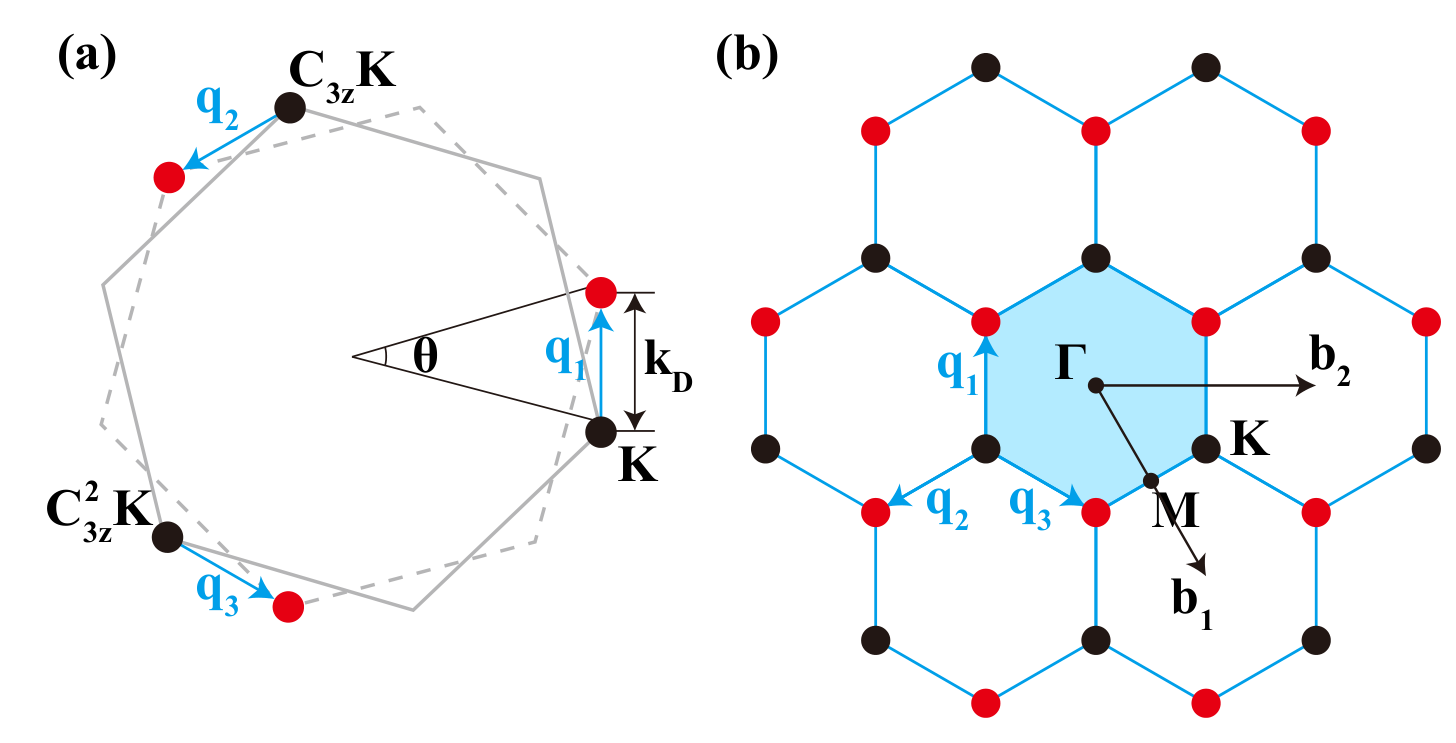
\includegraphics[width=0.8\linewidth]{fig/moire-vectors.png}
\caption{Momentum transfers \( \q_{\text{b}} \), \( \q_{\text{tr}} \), \( \q_{\text{tl}} \), and the \( \Q \)-lattice in the reciprocal moiré space.}
\label{fig:Q_lattice}
\end{figure}

Next, we redefine the momenta for layers 1 and 2 as
\begin{equation} \label{eq:redef_k1k2_momenta_Qlattice}
\q_1 = \k_1 - K_1 = \k - \Q_B, \quad \q_2 = \k_2 - K_2 = \k - \Q_A.
\end{equation}

Since $\q_2 - \q_1$ can assume the three values $\q_{\text{b}}$, $\q_{\text{tr}}$ or $\q_{\text{tl}}$, in the new representation the transfer rules become
\begin{align} \label{eq:selection_rules_qbqtrqtl_QAQB}
\begin{cases}
\; \q_2-\q_1=\q_{\text{b}}  \implies \Q_B = \Q_A + \q_{\textbf{b}} \\
\; \q_2-\q_1=\q_{\text{tr}} \implies \Q_B = \Q_A + \q_{\textbf{tr}} \\
\; \q_2-\q_1=\q_{\text{tl}} \implies \Q_B = \Q_A + \q_{\textbf{tl}}
\end{cases}
\end{align}

Within the $\Q$-lattice representation, combining Equations \ref{eq:single_layer_dirac_hamil_valley}, \ref{eq:interlayer-hopping-kspace}, and \ref{eq:interlayer-3terms}, the Bistritzer-MacDonald Hamiltonian for one single valley \( \zeta \), also referred to as MBM-1V \cite{all_magic_angles}, is given by:
\begin{equation} \label{eq:mbm-1v}
H^\zeta_{\Q\Q'}(\k) = \zeta v_F \delta_{\Q,\Q'} (\k - \Q) \vdot (\s_x, \zeta \s_y) +
w \sum_{j = \text{b},\text{tr},\text{tl}} \qty(\delta_{\Q'-\Q,\q_j} + \delta_{\Q-\Q',\q_j}) T_{j}^\zeta.
\end{equation}

By inserting the usual values \( \theta = 1.05^\circ \), \( v_F = 5.994 \, \unit{eV \cdot \AA} \), \( a = 2.46 \unit{\AA} \), \( w = 110 \unit{meV} \), and \( w_0 = 0.8 \, w \) \cite{topoheavyfermion2022}, and diagonalizing the Hamiltonian given in Equation \ref{eq:mbm-1v} for valley \( \zeta = +1 \), we obtain the band structure depicted in Figure \ref{fig:continuum_model_bands}.

\begin{figure}[H]
\centering
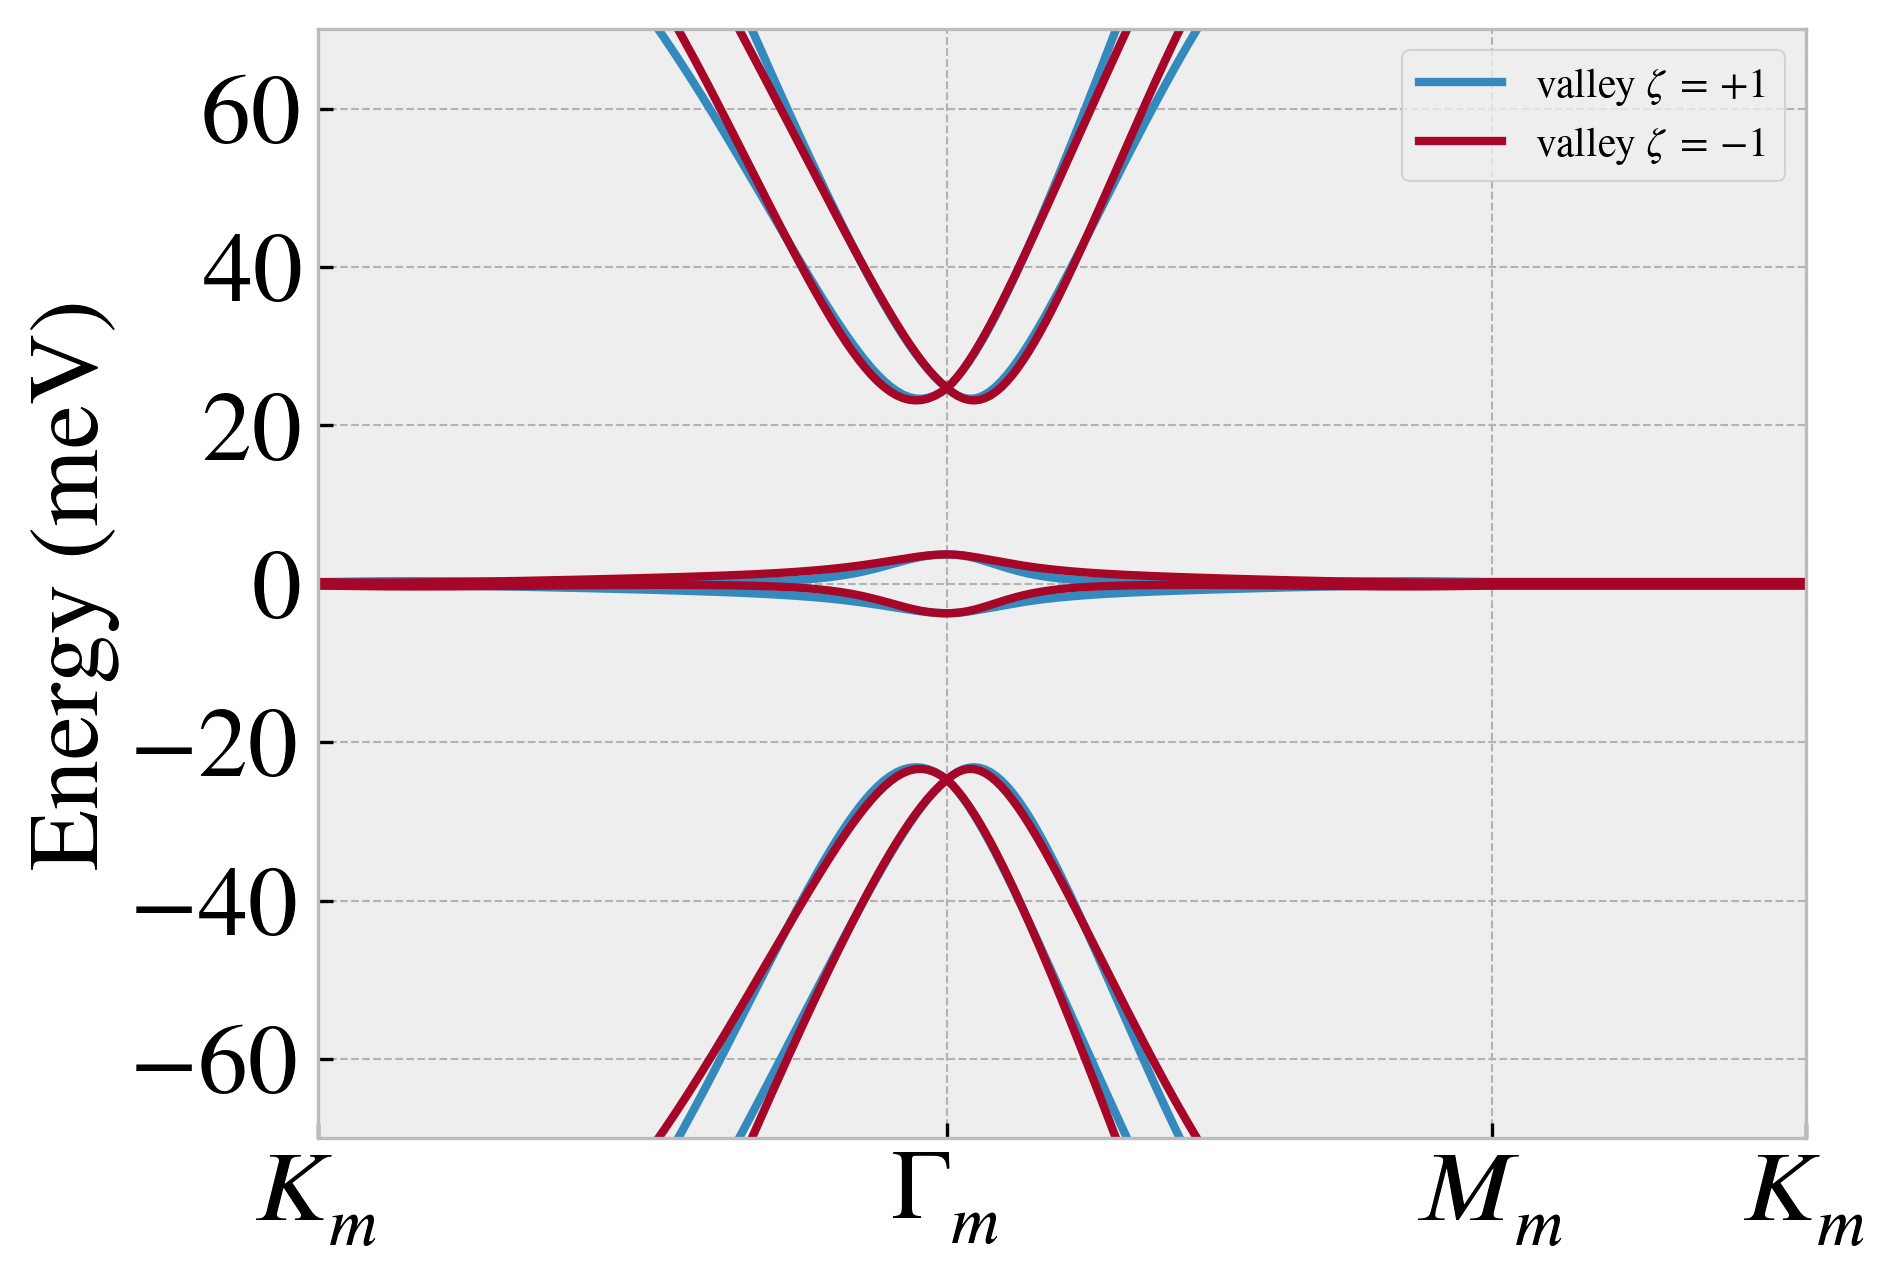
\includegraphics[width=0.8\linewidth]{fig/continuum_model_bands.png}
\caption{Continuum model energy spectrum for valley \( \zeta = +1 \). The energy range was zoomed in to emphasize the flat bands.}
\label{fig:continuum_model_bands}
\end{figure}


%%%%%%%%%%%%%%%%%%%%%%%%%%%%%%%%%%%%%%%%%%%%%%%%%%%%%%%%%%%%%%%%%%%%%%%%%%%%%%%%%%%%%%%%%%%%%%%%%%
\section{Symmetry analysis and Wannier obstruction} \label{sec:symmetry_analysis}
%%%%%%%%%%%%%%%%%%%%%%%%%%%%%%%%%%%%%%%%%%%%%%%%%%%%%%%%%%%%%%%%%%%%%%%%%%%%%%%%%%%%%%%%%%%%%%%%%%

As discussed in \cite{zou2018}, at currently accessible energy scales, experiments indicate that MATBG exhibits approximate emergent symmetries. These include translational symmetry characterized by the constant $L'(\theta) = a / (2 \sin\theta/2)$, valley symmetry $U_v(1)$, and $C_{6} T$, which are not fully captured by a generic commensurate structure described in Section \ref{sec:tbg_commensurate}. The continuum model in Section \ref{sec:BM-model} incorporates all these ``good'' symmetries. In this section, we will characterize the symmetries of the BM model that will later be analyzed to understand the Wannier Obstruction \cite{zou2018} and the Topological Heavy Fermion model of MATBG \cite{topoheavyfermion2022}.
In this section, we define $H = H_{\text{MBM-1V}}$, which refers to the Hamiltonian in Eq. \eqref{eq:mbm-1v}. \textbf{MELHORAR PARÁGRAFO}.

%%%%%%%%%%%%%%%%%%%%%%%%%%%%%%%%%%%%%%%%%%%%%%%%%%%%%%%%%%%%%%%%%%%%%%%%%%%%%%%%%%%%%%%%%%%%%%%%%%
\subsection{$U_v(1)$ valley symmetry} \label{subsec:Uv(1)-valley_symmetry}
%%%%%%%%%%%%%%%%%%%%%%%%%%%%%%%%%%%%%%%%%%%%%%%%%%%%%%%%%%%%%%%%%%%%%%%%%%%%%%%%%%%%%%%%%%%%%%%%%%

The double degeneracy of the flat bands at \( \Gamma_m \), as seen in Figure \ref{fig:continuum_model_bands}, is not a typical feature but rather an accidental one \cite{thesis_angeli}. This degeneracy arises from the effective suppression of interlayer coupling between Dirac points of different valleys at small twist angles, despite symmetry not explicitly forbidding such couplings. This phenomenon is attributed to an emergent symmetry, often referred to as valley charge conservation or the \( U_v(1) \) symmetry.

At small twist angles, the matrix element of the single-layer component of the Hamiltonian becomes negligibly small, leading to an effective decoupling of the valleys from one another. This decoupling implies that the operator
\begin{equation} \label{eq:Uv(1)_symmetry_N1N2}
\Delta N_v = N_1 - N_2,
\end{equation}
where \( N_1 \) and \( N_2 \) represent the occupation numbers of each valley, commutes with the non-interacting Hamiltonian at small angles. This operator acts as the generator of the emergent \( U_v(1) \) symmetry.


%%%%%%%%%%%%%%%%%%%%%%%%%%%%%%%%%%%%%%%%%%%%%%%%%%%%%%%%%%%%%%%%%%%%%%%%%%%%%%%%%%%%%%%%%%%%%%%%%%
\subsection{Magnetic point group symmetries} \label{subsec:magnetic_point_group_symmetries}
%%%%%%%%%%%%%%%%%%%%%%%%%%%%%%%%%%%%%%%%%%%%%%%%%%%%%%%%%%%%%%%%%%%%%%%%%%%%%%%%%%%%%%%%%%%%%%%%%%

First of all, we would like to emphasize that spin-orbit coupling (SOC) is completely neglected in the model presented in Eq. \eqref{eq:mbm-1v}, as it is negligible in graphene itself. Additionally, when we refer to time-reversal symmetry, we are specifically referring to the spinless version.

The MBM-1V model exhibits symmetry properties distinct from the intuitive candidate magnetic space group \( P6221' \), which corresponds to the honeycomb lattice space group with a \( D_6 \) point group combined with time-reversal \( T \). These differences arise due to the absence of inter-valley coupling between the \( K \) and \( K' \) Dirac points, from the $U_v(1)$ symmetry. This absence breaks certain symmetries inherent in the original graphene lattice, including time-reversal \( T \) and the rotational symmetries \( C_{6z} \) and \( C_{2y} \), while preserving \( C_{3z} \).

As a result, the symmetry group of the MBM-1V model is identified as the magnetic space group \( P6'2'2 \) (\#177.151 in BNS notation \cite{bilbao_1}). This group incorporates the symmetries \( C_{6z}T \), \( C_{2y}T \), and \( C_{2x} \), which satisfy the algebraic relations \( (C_{6z}T)^2 = C_{3z} \), \( (C_{6z}T)^3 = C_{2z}T \), and $C_{2y} T = (C_{2z}T) C_{2x}$.

The MBM-1V Hamiltonian, given in Eq.~\eqref{eq:mbm-1v}, is constructed from the Dirac states near the \( K \) point of the top and bottom graphene layers, excluding contributions from the \( K' \) cone. Consequently, the states at \( K' \) form a separate, time-reversed MBM-1V system, breaking explicit time-reversal symmetry in the one-valley model. However, the MBM-1V Hamiltonian retains invariance under the combined anti-unitary operation \( C_{2z}T \), which is in the magnetic space group \( P6'2'2 \).

The point group \( 6'2'2 \), as geometrically depicted in Figure \ref{fig:622_magnetic}, can be generated by the following symmetries, where their operators are represented in the \( \Q \)-lattice by matrix elements \( D_{\Q',\Q} \) \cite{all_magic_angles}. To simplify notation, we label $\q_1 = \q_{\text{b}}$, $\q_2 = \q_{\text{tr}}$, and $\q_3 = \q_{\text{tl}}$.
\begin{itemize}
\item \( C_{3z} \):
\begin{equation} \label{eq:C3z_Qlattice_mbm1v}
H_{\text{MBM-1V}}(\mathbf{k}) = D^\dagger(C_{3z}) H_{\text{MBM-1V}}(C_{3z}\mathbf{k}) D(C_{3z}),
\end{equation}
\begin{equation}
D_{\Q',\Q}(C_{3z}) = e^{i\frac{2\pi}{3}\sigma_z} \delta_{\Q',C_{3z}\Q}, \quad C_{3z}\q_j = \q_{j+1}.
\end{equation}

\item \( C_{2x} \):
\begin{equation} \label{eq:C2x_Qlattice_mbm1v}
H_{\text{MBM-1V}}(\mathbf{k}) = D^\dagger(C_{2x}) H_{\text{MBM-1V}}(C_{2x}\mathbf{k}) D(C_{2x}),
\end{equation}
\begin{equation}
D_{\Q',\Q}(C_{2x}) = \sigma_x \delta_{\Q',C_{2x}\Q}, \quad C_{2x}\q_1 = -\q_1, \quad C_{2x}\q_2 = -\q_3, \quad C_{2x}\q_3 = -\q_2.
\end{equation}

\item \( C_{2z}T \):
\begin{equation} \label{eq:C2zT_Qlattice_mbm1v}
H_{\text{MBM-1V}}(\mathbf{k}) = D(C_{2z}T) H_{\text{MBM-1V}}^*(\mathbf{k}) D^T(C_{2z}T),
\end{equation}
\begin{equation}
D_{\Q',\Q}(C_{2z}T) = \sigma_x \delta_{\Q',\Q}.
\end{equation}
\end{itemize}

In the real-space basis of the Hamiltonian \( H_{\text{MBM-1V}}(\r) \), these symmetries are more conveniently represented in terms of valley (\( \tau \)) and sublattice (\( \sigma \)) degrees of freedom \cite{bernevig_II_2021}. Specifically, we have \( C_{2z}T = \sigma_x \mathcal{K} \), where \( \mathcal{K} \) denotes complex conjugation, \( C_{3z} = e^{i\frac{2\pi}{3} \sigma_z} \), and \( C_{2x} = \tau_x \sigma_x \).


%%%%%%%%%%%%%%%%%%%%%%%%%%%%%%%%%%%%%%%%%%%%%%%%%%%%%%%%%%%%%%%%%%%%%%%%%%%%%%%%%%%%%%%%%%%%%%%%%%
\subsection{Particle-hole symmetry} \label{subsec:ph_symmetry}
%%%%%%%%%%%%%%%%%%%%%%%%%%%%%%%%%%%%%%%%%%%%%%%%%%%%%%%%%%%%%%%%%%%%%%%%%%%%%%%%%%%%%%%%%%%%%%%%%%

The MBM-1V model features an approximate \textit{particle-hole} (PH) symmetry $P$, derived from the PH symmetry inherent to the low-energy Dirac nodes in monolayer graphene.  This symmetry is a central aspect of understanding the band topology in the model \cite{all_magic_angles}. However, it is not exact and can be broken under specific conditions. For instance, regarding \( H_{\ell}^\zeta \), deviations arise due to the inclusion of \(\theta\)-dependent terms (as we saw in Equation \ref{eq:single_layer_dirac_hamil_valley}), which disrupt the symmetry. Additionally, higher-order momentum corrections, such as \( k^2 \)-dependent terms, break the PH symmetry originally present in the Dirac nodes.

Despite these breaking mechanisms, the particle-hole (PH) symmetry remains a useful approximation for analyzing the band topology. The corresponding operator \( P \) is unitary and satisfies the algebra \cite{bernevig_II_2021}:
\begin{equation} \label{eq:PH_symmetry_algebra}
[P, C_{2z}T] = [P, C_{3z}] = 0, \quad \{P, C_{2x}\} = 0, \quad P^2 = -1,
\end{equation}
where its representation in the valley-sublattice degrees of freedom is given by \( P = i \tau_x \sigma_y \), with \( \tau_x \) being the Pauli matrix associated with the \( x \)-component of the valley degree of freedom.

Within the $\Q$-lattice, $P$ can be mathematically expressed as \cite{all_magic_angles}:
\begin{equation} \label{eq:ph_symmetry_hamiltonian}
H_{\text{MBM-1V}}(\mathbf{k}) = -D^\dagger(P) H_{\text{MBM-1V}}(-\mathbf{k}) D(P),
\end{equation}
The matrix \( D_{\Q',\Q}(P) \) is defined as:
\begin{equation} \label{eq:D(P)_Q_lattice_PH_symmetry}
D_{\Q',\Q}(P) = \delta_{\Q',-\Q} \zeta_\Q,
\end{equation}
with \( \zeta_\Q = 1 \) assigned to \( \Q_A \) vectors, while \( \zeta_\Q = -1 \) corresponds to \( \Q_B \) vectors. Note that \( \Q_A \) and \( \Q_B \) correspond to the black and red circles, respectively, as depicted in Figure \ref{fig:Q_lattice}.

%%%%%%%%%%%%%%%%%%%%%%%%%%%%%%%%%%%%%%%%%%%%%%%%%%%%%%%%%%%%%%%%%%%%%%%%%%%%%%%%%%%%%%%%%%%%%%%%%%
\subsection{Representations of the two middle bands} \label{subsec:reps_two_middle_bands}
%%%%%%%%%%%%%%%%%%%%%%%%%%%%%%%%%%%%%%%%%%%%%%%%%%%%%%%%%%%%%%%%%%%%%%%%%%%%%%%%%%%%%%%%%%%%%%%%%%

By utilizing the \texttt{COREPRESENTATIONS} tool from the Bilbao Crystallographic Server \cite{bilbao_1} for the magnetic space group \( P6'2'2 \) (\#177.151 in BNS notation), we determine the irreducible co-representations (irreps) at the high-symmetry momenta \(\Gamma_m\), \(K_m\), and \(M_m\). Given that twisted bilayer graphene is considered spinless, double groups are not relevant in this context, and irreps ``with bars'', such as \(\overline{\Gamma}_4\), can be disregarded. As a result, the allowed irreps are \(\Gamma_1\), \(\Gamma_2\), and \(\Gamma_3\) at \(\Gamma_m\); \(M_1\) and \(M_2\) at \(M_m\); and \(K_1\) and \(K_2K_3\) at \(K_m\). The corresponding character tables for these irreps are provided in Table \ref{tab:P6'2'2_characters}.

\begin{table}[H]
\caption{Character table of irreps at high symmetry momenta in magnetic space group $P6'2'2$.}
\centering
\begin{tabular} { c c c c | c c c | c c c }
\cline{1-10}
$\P$ & $\P \Gamma_1$ & $\P \Gamma_2$ & $\P \Gamma_3$ & $\P$ & $\P M_1$ & $\P M_2$ & $\P$ & $\P K_1$ & $\P K_2K_3$ \\
\cline{1-10}
$E$ & $\P1$ & $\P1$ & $\P2$ & $\P E$ & $\P1$ & $\P1$ & $\P E$ & $\P1$ & $\P2$ \\
$2 C_3$ & $\P1$ & $\P1$ & $ -1$ & $\P C_2'$ & $\P1$ & $ -1$ & $\P C_3$ & $\P1$ & $ -1$ \\
$3 C_2'$ & $\P1$ & $ -1$ & $\P0$ & $\P$ & $\P$ & $\P$ & $\P C_3^{-1}$ & $\P1$ & $-1$ \\
\cline{1-10}
\end{tabular}
\label{tab:P6'2'2_characters}
\end{table}

In Table \ref{tab:P6'2'2_characters}, all the irreducible co-reps are induced from the irreps of the corresponding high-symmetry momenta in the unitary subspace group \( P312 \) (\#149) \cite{all_magic_angles, bradley_representation_theory_2010}, which can be read from the Bilbao server \cite{bilbao_1}. For instance, consider the \( K_m \) point. In \( P312 \), the \( K_m \) point has three one-dimensional irreps: \( K_1 \), \( K_2 \), and \( K_3 \). Here, \( K_1 \) is real, while \( K_2 \) and \( K_3 \) are complex conjugates of each other. Under the action of the \( C_{2z}T \) symmetry, \( K_1 \) remains invariant, whereas \( K_2 \) and \( K_3 \) are interchanged due to complex conjugation. Consequently, in \( P6'2'2 \), \( K_1 \) forms an independent co-rep, while \( K_2 \) and \( K_3 \) combine to form a co-rep denoted as \( K_2K_3 \).

Next, we sketch the proof from \cite{all_magic_angles} that the middle two bands in the system, whenever they are gapped, form the irreps \(\Gamma_1 \oplus \Gamma_2\), \(M_1 \oplus M_2\), and \(K_2K_3\). This result holds for any value of \(w\) in the Hamiltonian defined by Eq.~\eqref{eq:mbm-1v}, provided the magnetic space group \(P6'2'2\) and the particle-hole symmetry \(P\) are included.

\begin{itemize}
\item $K_m$ point:

First of all, we prove that the irrep \(K_2K_3\) at the point \(K_m\) is pinned at zero energy. The little group of \(K_m\) contains the symmetries \(C_{3z}\), \(C_{2z}T\), and \(PC_{2x}\). These symmetries satisfy the relations:
\begin{equation} \label{eq:proof_flatbands_Km_point_1}
[C_{3z}, C_{2z}T] = 0, \quad C_{3z}(PC_{2x}) = (PC_{2x})C_{3z}^{-1} , \quad [C_{2z}T, PC_{2x}] = 0.
\end{equation}

From the character table \ref{tab:P6'2'2_characters}, we select the \(C_{3z}\) eigenstates for a basis for \(K_2K_3\):
\begin{equation} \label{eq:proof_flatbands_Km_point_2}
C_{3z} |1\rangle = e^{i \frac{2\pi}{3}} |1\rangle, \quad C_{3z} |\bar{1}\rangle = e^{-i \frac{2\pi}{3}} |\bar{1}\rangle.
\end{equation}

The symmetry \(PC_{2x}\) flips the \(C_{3z}\) eigenvalue:
\begin{equation} \label{eq:proof_flatbands_Km_point_2}
C_{3z}\qty(PC_{2x} |1\rangle) = PC_{2x}C_{3z}^{-1} |1\rangle = e^{-i \frac{2\pi}{3}} \qty(PC_{2x} |1\rangle).
\end{equation}
Additionally, \(PC_{2x}\) anti-commutes with the Hamiltonian at $K_m$. If $H(K_m) \ket{1} = \eps \ket{1}$, then $PC_{2x} \ket{1}$ is an eigenstate of $H(K_m)$ with opposite eigenvalue $-\eps$:
\begin{equation} \label{eq:proof_flatbands_Km_point_2}
H(K_m) \qty(PC_{2x} |1\rangle) = -PC_{2x} H(K_m) |1\rangle = -\epsilon \qty(PC_{2x} |1\rangle).
\end{equation}
This leads to two cases:
\begin{enumerate}[label=(\Roman*)]
\item \(\epsilon = 0\), where \(|\bar{1}\rangle = PC_{2x} |1\rangle\), indicating that the states are related by particle-hole symmetry and lie at zero energy.
\item \(\epsilon \neq 0\), where \(|\bar{1}\rangle \neq PC_{2x} |1\rangle\), and \(PC_{2x} |1\rangle\) forms a state with opposite energy, \(-\epsilon\).
\end{enumerate}

In case (II), the states \(PC_{2x} |1\rangle\) and \(C_{2z}T \qty(PC_{2x} |1\rangle)\) together form another \(K_2K_3\) irrep at opposite energy \(-\epsilon\). As a result, the \(K_2K_3\) irrep can either appear in pairs with opposite energy eigenvalues or appear alone at zero energy.

In the \(w = 0\) limit, where there is no interlayer hybridization, the Hamiltonian \(H(K_m)\) has two zero-energy eigenstates forming a \(K_2K_3\) irrep. Upon increasing \(w\), the system undergoes a continuous transformation while preserving particle-hole symmetry. Such a transformation cannot shift a single \(K_2K_3\) irrep away from zero energy in a PH-symmetric manner. Consequently, case (I) prevails: a single \(K_2K_3\) irrep is constrained to remain at zero energy.

\item $\Gamma_m$ point:

Here we prove that the middle two bands, when gapped, form \(\Gamma_1 \oplus \Gamma_2\) irreps at \(\Gamma_m\). While the two-dimensional irrep \(\Gamma_3\) could, in principle, represent the middle two bands if they are degenerate, this is prohibited in the MBM-1V Hamiltonian at Eq. \eqref{eq:mbm-1v} with PH symmetry. The little group of the \(\Gamma_m\) point has the symmetries \(C_{3z}\), \(C_{2x}\), \(C_{2z}T\), and \(P\), which satisfy:
\begin{equation} \label{eq:proof_flatbands_GMm_point_1}
C_{2x}C_{3z}C_{2x}^{-1} = C_{3z}^{-1}, \quad [C_{3z}, C_{2z}T] = 0, \quad [C_{3z}, P] = 0,
\end{equation}
\begin{equation} \label{eq:proof_flatbands_GMm_point_2}
[C_{2x}, C_{2z}T] = 0, \quad \{C_{2x}, P\} = 0, \quad [C_{2z}T, P] = 0.
\end{equation}

Since \( \Gamma_3 \) shares the same \( C_{3z} \) eigenvalues as \( K_2K_3 \) (as shown in Table \ref{tab:P6'2'2_characters}), the same reasoning applies. Thus, similar to \( K_2K_3 \), the \( \Gamma_3 \) irrep either appears in pairs with opposite energies or at zero energy. However, in the case of the Hamiltonian \( H(\Gamma_m) \) with \( w = 0 \), there is no zero eigenvalue. Additionally, no process preserving particle-hole symmetry can generate a single zero mode. As a result, \( \Gamma_3 \) can only appear in pairs, and each of the middle two bands must actually form \( \Gamma_1 \) or \( \Gamma_2 \) irreps.

Next, we show that these two bands have opposite energy eigenvalues due to \( P \)-symmetry. Suppose \( |\Gamma_1\rangle \) has a \( C_{2x} \) eigenvalue of \( +1 \) and an energy \( \epsilon \). Using the anti-commutation relations \( \{C_{2x}, P\} = 0 \) and \( \{H(\Gamma_m), P\} = 0 \), it follows that \( P |\Gamma_1\rangle \) has a \( C_{2x} \) eigenvalue of \( -1 \) and an energy eigenvalue of \( -\epsilon \). Consequently, \( P |\Gamma_1\rangle \) forms a \( \Gamma_2 \) irrep at energy \( -\epsilon \). Therefore, we conclude that the gapped middle two bands always form the direct sum of irreps \( \Gamma_1 \oplus \Gamma_2 \) at \( \Gamma_m \).

\item $M_m$ point:

At the \(M\) point, the middle two bands form \(M_1 \oplus M_2\) irreps. The little group of the \(M\) point has the symmetries \(C_2' = C_{3z}C_{2x}C_{3z}^{-1}\), \(C_{2z}T\), and \(P\), which satisfy:
\[
[C_2', C_{2z}T] = 0, \quad \{C_2', P\} = 0, \quad [C_{2z}T, P] = 0.
\]
The irreps \(M_1\) and \(M_2\) have \(C_{2x}\) eigenvalues of \(+1\) and \(-1\), respectively, and, similar to \(\Gamma_1 \oplus \Gamma_2\), they appear in pairs due to the anti-commutation relation \(\{C_2', P\} = 0\).

\end{itemize}

In conclusion, this establishes that the gapped middle two bands must inevitably form the irreps \( \Gamma_1 \oplus \Gamma_2 \), \( M_1 \oplus M_2 \), and \( K_2K_3 \).




%%%%%%%%%%%%%%%%%%%%%%%%%%%%%%%%%%%%%%%%%%%%%%%%%%%%%%%%%%%%%%%%%%%%%%%%%%%%%%%%%%%%%%%%%%%%%%%%%%
\subsection{Wannier obstruction} \label{subsec:wannier_obstruction_mbm_1v}
%%%%%%%%%%%%%%%%%%%%%%%%%%%%%%%%%%%%%%%%%%%%%%%%%%%%%%%%%%%%%%%%%%%%%%%%%%%%%%%%%%%%%%%%%%%%%%%%%%

The Elementary Band Representations (EBRs) for the magnetic space group \( P6'2'2 \) are readily accessible through the \texttt{MBANDREP} program on the Bilbao Crystallographic Server \cite{bilbao_1, bilbao_2}. In Table \ref{tab:P6'2'2-ebrs}, we present only the maximal Wyckoff positions and inductions from single-valued irreps, as double groups are not relevant to our analysis.

\begin{table}[H]
\footnotesize
\caption{Elementary band representations for the magnetic space group \( P6'2'2 \). The first row lists the Wyckoff positions. The second row provides the corresponding site-symmetry groups and their unitary subgroups. In the third row, \( G_\rho^q = \rho \uparrow G \) denotes the elementary band representation (EBR) generated from the co-rep \( \rho \) of the site-symmetry group at Wyckoff position \( q \), with the dimension of each EBR indicated in parentheses. The co-reps \( \rho \) are induced from the irreps of the unitary subgroups \cite{bradley_representation_theory_2010}, which can be accessed at the Bilbao server \cite{bilbao_1}. The fourth to sixth rows provide the decomposition of $G_\rho^q$ into irreps of the little groups at high-symmetry momenta $\Gamma$, $K$ and $M$ (Equation \ref{eq:induce_subduce}).}
\centering
\begin{tabular}{|c|c|c|c|c|c|c|c|c|}
\hline
Wyckoff pos. & \multicolumn{3}{c|}{$1a$} & \multicolumn{3}{c|}{$2c$} & \multicolumn{2}{c|}{$3f$} \\
\cline{1-9}
Site sym. & \multicolumn{3}{c|}{$6'2'2$, $32$} & \multicolumn{3}{c|}{$32$, $32$} & \multicolumn{2}{c|}{$2'2'2$, $2$} \\
\cline{1-9}
EBR & $G_{A_1}^{1a}(1)$ & $G_{A_2}^{1a}(1)$ & $G_{E}^{1a}(2)$ & $G_{A_1}^{2c}(2)$ & $G_{A_2}^{2c}(2)$ & $G_{E}^{2c}(4)$   & $G_{A}^{3f}(3)$ & $G_{B}^{3f}(3)$ \\
\hline
$\Gamma$ & $\Gamma_1$ & $\Gamma_2$ & $\Gamma_3$ & $2\Gamma_1$ & $2\Gamma_2$ & $2\Gamma_3$ & $\Gamma_1\oplus \Gamma_3$ & $\Gamma_2\oplus \Gamma_3$ \\
\hline
$K$ & $K_1$ & $K_1$ & $K_2 K_3$ & $K_2 K_3$ & $K_2 K_3$ & $2K_1 \oplus  K_2 K_3$ & $K_1\oplus K_2 K_3$ & $K_1\oplus K_2 K_3$ \\
\hline
$M$ & $M_1$ & $M_2$ & $M_1\oplus M_2$ & $2M_1$ & $2M_2$ & $2M_1\oplus 2M_2$ & $2M_1\oplus M_2$ & $M_1\oplus 2M_2$ \\
\hline
\end{tabular}
\label{tab:P6'2'2-ebrs}
\end{table}

On Table \ref{tab:P6'2'2-ebrs}, we emphasize that each Wyckoff position in the Moiré pattern corresponds to a distinct region. For instance, the \( 1a \) and \( 2c \) Wyckoff positions correspond to the AA-stacking and AB-stacking regions, respectively.

As demonstrated in Section \ref{subsec:reps_two_middle_bands}, incorporating the approximate particle-hole symmetry $P$ within the single valley Bistritzer-MacDonald model ensures that the middle two flat bands in each valley align with the irreducible co-representations (irreps)
\begin{equation} \label{eq:matbg-irreps}
\Gamma_1(1) \oplus \Gamma_2(1); \; M_1(1) \oplus M_2(1); \; K_2 K_3(2),
\end{equation}
of the magnetic space group \( P6'2'2 \), with their characters shown in Table \ref{tab:P6'2'2_characters}.

We now show that the middle two bands exhibit at least fragile topology, with this result relying crucially on particle-hole (PH) symmetry. Without this symmetry, it is not possible to demonstrate that the gapped bands around the charge neutrality point are topological \cite{all_magic_angles}.

From Table \ref{tab:P6'2'2-ebrs}, we note that the representations of the two middle bands in Eq. \eqref{eq:matbg-irreps} cannot be expressed as a positive sum of EBRs. Instead, they can only be written as a difference of EBRs:
\begin{equation} \label{eq:matbg-difference_of_ebrs}
G_{2c}^{A_1} + G_{1a}^{A_2} - G_{1a}^{A_1}.
\end{equation}

This fact suggests the presence of \textit{at least fragile topology}. By analyzing the representation content, one might consider adding the ``negative'' band \( G_{1a}^{A_1} \) and coupling it with the middle two bands of MBM-1V. In this case, the three bands could be interpreted as a sum of EBRs, resulting in a trivial system. This scenario exemplifies fragile topology \cite{FragileTopology_Po2018}, where the topology can be trivialized by the addition of a trivial band. However, the system retains the key feature of not being representable by exponentially localized Wannier functions, reflecting a Wannier obstruction that defines its non-trivial topological nature.

In conclusion, particle-hole symmetry in MBM-1V ensures the presence of non-trivial topology. Notably, the ``at least fragile topology,'' when PH symmetry is included, was actually demonstrated in \cite{bernevig_II_2021} to be a stable topology protected by the combined symmetry \( \mathcal{P} = P C_{2z}T \). They derived this result using the concept of Wilson loops, which is beyond the scope of this thesis. In the absence of PH symmetry, the topology remains fragile, being protected by the \( C_{2z}T \) symmetry \cite{faithful_fragile_topology_po2019}.

%%%%%%%%%%%%%%%%%%%%%%%%%%%%%%%%%%%%%%%%%%%%%%%%%%%%%%%%%%%%%%%%%%%%%%%%%%%%%%%%%%%%%%%%%%%%%%%%%%
%%%%%%%%%%%%%%%%%%%%%%%%%%%%%%%%%%%%%%%%%%%%%%%%%%%%%%%%%%%%%%%%%%%%%%%%%%%%%%%%%%%%%%%%%%%%%%%%%%


%%%%%%%%%%%%%%%%%%%%%%%%%%%%%%%% COMMENT THIS TO COMPILE main.tex %%%%%%%%%%%%%%%%%%%%%%%%%%%%%%%%
%%-----
%% Referências bibliográficas
%%-----
\addcontentsline{toc}{chapter}{\bibname}
%\bibliographystyle{abntex2-num}
\bibliography{citations}
\bibliographystyle{ieeetr}
\end{document}
%%%%%%%%%%%%%%%%%%%%%%%%%%%%%%%% COMMENT THIS TO COMPILE main.tex %%%%%%%%%%%%%%%%%%%%%%%%%%%%%%%%
